\documentclass{article}

\usepackage[letterpaper, portrait, margin=1in]{geometry}
\usepackage{tikz}
\usepackage{mathtools}
\usetikzlibrary{shapes,backgrounds}
\usepackage{amsmath}
\begin{document}

\title{Dyanmics Equations for Smartmouse 2018}
\author{Peter Mitrano}

\maketitle

Deriving the kinematic equations of a differential drive robot.

\hfill

\begin{figure}[h]
  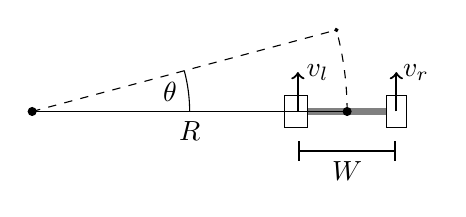
\begin{tikzpicture}
    \draw [line width=1mm, draw=gray]{(3.5,0)--(4.5, 0)};
    \draw {(3.2,-0.2) rectangle (3.5, 0.2)};
    \draw {(4.5,-0.2) rectangle (4.75, 0.2)};
    \draw  {(0,0) -- (4, 0)};
    \draw [dashed, rotate around={15:(0,0)}] {(0,0) -- (4, 0)};
    \draw [dashed] (4,0) arc (0:15:4);
    \draw (2,0) arc (0:15:2);
    \draw [thick,->] (3.375,0) -- (3.375,0.5);
    \draw [thick,->] (4.625,0) -- (4.625,0.5);
    \draw [thick,|-|] (3.375,-0.5) -- (4.625,-0.5);
    \filldraw {(0,0) circle (.05)};
    \filldraw {(4,0) circle (.05)};
    \filldraw [rotate around={15:(0,0)}]{(4,0) circle (.02)};
    \draw (1.75, 0.25) node {$\theta$};
    \draw (3.625, 0.5) node {$v_l$};
    \draw (4.875, 0.5) node {$v_r$};
    \draw (2, -0.25) node {$R$};
    \draw (4, -0.75) node {$W$};
  \end{tikzpicture}
  \centering
\end{figure}

At an instant in time we say that the robot is turning around some point ICC, the instanteous center. The radius $R$ about that point is what we want to solve for. We start with the knowedge that since the robot doesn't tear itself apart while driving, the rate $w$ at which both wheels (and the robot) move around that center is the same.
\begin{equation} \label{eq:1}
  \omega_l = \omega_r = w
\end{equation}
Let $R_l$ and $R_l$ be the radius to the right and left wheels.
\begin{equation} \label{eq:2}
  \omega_l = \frac{v_l}{R_l}, \omega_r = \frac{v_r}{R_r}
\end{equation}
We can then combine \ref{eq:1} and \ref{eq:2}
\begin{equation}
  \frac{v_l}{R_l} = \frac{v_r}{R_r}
\end{equation}
We can then substitute $R_l = R - \frac{w}{2}$ and $R_r = R + \frac{w}{2}$
\begin{equation}
  \frac{v_l}{R-\frac{w}{2}} = \frac{v_r}{R + \frac{w}{2}}
\end{equation}

No do some algebra...
\begin{align*}
  \frac{v_l}{R-\frac{w}{2}} &= \frac{v_r}{R + \frac{w}{2}} \\[1em]
  \frac{R-\frac{w}{2}}{v_l} &= \frac{R + \frac{w}{2}}{v_r} \\[1em]
  \frac{R}{v_l}-\frac{w}{2v_l} &= \frac{R}{v_r} + \frac{w}{2v_r} \\[1em]
  \frac{R}{v_l}-\frac{R}{v_r} &= \frac{w}{2v_r}+\frac{w}{2v_l} \\[1em]
  \frac{R(v_r-v_l)}{v_rv_l} &= \frac{w(v_l+v_r)}{2v_rv_l} \\[1em]
  R(v_r-v_l) &= w(v_l+v_r) \\[1em]
  R &= \frac{w(v_l+v_r)}{2(v_r-v_l)} \\[1em]
\end{align*}

\textbf{mic drop.}

\end{document}

